\documentclass[conference]{IEEEtran}
\usepackage[utf8]{inputenc}
\usepackage[T5]{fontenc}
\usepackage[english,vietnamese]{babel}
\usepackage{lmodern}
\usepackage{amsmath,amssymb,booktabs,graphicx,microtype}
\usepackage{algpseudocode}
\usepackage{tikz}
\usetikzlibrary{arrows.meta,positioning}
\usepackage[hidelinks]{hyperref}
\graphicspath{{../results/e1/figures/}{../results/e3/figures/}}

\newcommand{\NMI}{\mathrm{NMI}}
\newcommand{\ARI}{\mathrm{ARI}}
\newcommand{\ACC}{\mathrm{ACC}}
% Sinh bởi scripts/report_tables.py từ CSV.
\newcommand{\EoneTable}{%
\begin{tabular}{llrrr}
\toprule
Họ & Thuật toán & Giây & Lượt/đỉnh & Cụm \\
\midrule
BA & FLPA FIFO & $5.223\pm1.672$ & $9.6$ & $1.0$ \\
BA & Leiden & $27.386\pm6.472$ & -- & $21.9$ \\
BA & LPA & $6.679\pm2.780$ & $15.7$ & $1.0$ \\
BA & Retention-LPA & $1.738\pm0.514$ & $4.3$ & $27403.4$ \\
ER & FLPA FIFO & $6.435\pm0.765$ & $29.8$ & $6.3$ \\
ER & Leiden & $12.531\pm2.570$ & -- & $27.1$ \\
ER & LPA & $10.190\pm4.980$ & $44.3$ & $6.3$ \\
ER & Retention-LPA & $0.831\pm0.149$ & $4.0$ & $31146.7$ \\
SBM & FLPA FIFO & $16.394\pm4.953$ & $32.8$ & $5.8$ \\
SBM & Leiden & $31.046\pm12.829$ & -- & $20.4$ \\
SBM & LPA & $23.648\pm13.024$ & $43.2$ & $5.7$ \\
SBM & Retention-LPA & $2.373\pm1.147$ & $4.7$ & $31029.0$ \\
\bottomrule
\end{tabular}}
\newcommand{\EthreeTable}{%
\begin{tabular}{rlrrrrrrr}
\toprule
$\mu$ & Biến thể & Giây & Lượt & Đổi nhãn & NMI & ARI & ACC & Cụm \\
\midrule
$0.30$ & FLPA FIFO & $0.029\pm0.001$ & $18293$ & $9416$ & $0.990\pm0.003$ & $0.972\pm0.011$ & $0.966\pm0.016$ & $108.7$ \\
$0.30$ & FIFO toàn bộ & $0.032\pm0.001$ & $21681$ & $9448$ & $0.991\pm0.002$ & $0.977\pm0.006$ & $0.973\pm0.009$ & $106.4$ \\
$0.30$ & FLPA LIFO & $0.070\pm0.003$ & $43296$ & $18482$ & $0.994\pm0.002$ & $0.982\pm0.010$ & $0.985\pm0.011$ & $100.2$ \\
$0.45$ & FLPA FIFO & $0.042\pm0.002$ & $26258$ & $11430$ & $0.961\pm0.005$ & $0.903\pm0.016$ & $0.916\pm0.019$ & $115.1$ \\
$0.45$ & FIFO toàn bộ & $0.044\pm0.002$ & $28964$ & $11385$ & $0.958\pm0.004$ & $0.901\pm0.011$ & $0.915\pm0.012$ & $117.6$ \\
$0.45$ & FLPA LIFO & $0.183\pm0.008$ & $111890$ & $42121$ & $0.967\pm0.005$ & $0.911\pm0.038$ & $0.939\pm0.017$ & $105.6$ \\
$0.60$ & FLPA FIFO & $0.086\pm0.008$ & $53534$ & $21036$ & $0.073\pm0.231$ & $0.043\pm0.136$ & $0.072\pm0.195$ & $12.4$ \\
$0.60$ & FIFO toàn bộ & $0.101\pm0.015$ & $64768$ & $21174$ & $0.077\pm0.242$ & $0.050\pm0.158$ & $0.076\pm0.210$ & $13.4$ \\
$0.60$ & FLPA LIFO & $0.410\pm0.066$ & $222809$ & $95197$ & $0.000\pm0.000$ & $0.000\pm0.000$ & $0.010\pm0.000$ & $1.0$ \\
\bottomrule
\end{tabular}}
\newcommand{\PaperTable}{%
\begin{tabular}{llrrr}
\toprule
Họ & Thuật toán & Paper (s) & Python (s) & $\Delta$ (\%) \\
\midrule
ER & LPA & $1.85$ & $3.076\pm0.276$ & $66$ \\
ER & Retention-LPA & $0.10$ & $0.316\pm0.014$ & $216$ \\
ER & FLPA FIFO & $0.85$ & $2.095\pm0.222$ & $146$ \\
ER & Leiden & $1.55$ & $6.143\pm0.642$ & $296$ \\
BA & LPA & $0.75$ & $3.606\pm1.471$ & $381$ \\
BA & Retention-LPA & $0.15$ & $1.166\pm0.404$ & $677$ \\
BA & FLPA FIFO & $0.35$ & $2.544\pm0.669$ & $627$ \\
BA & Leiden & $1.80$ & $16.328\pm2.721$ & $807$ \\
SBM & LPA & $1.75$ & $8.446\pm2.480$ & $383$ \\
SBM & Retention-LPA & $0.15$ & $1.288\pm0.349$ & $758$ \\
SBM & FLPA FIFO & $0.80$ & $6.474\pm2.448$ & $709$ \\
SBM & Leiden & $1.25$ & $14.978\pm3.400$ & $1098$ \\
\bottomrule
\end{tabular}}
\newcommand{\AuthorTable}{%
\begin{tabular}{llrrrr}
\toprule
Họ & Thuật toán & Cặp & C (s) & Python (s) & $\Delta$ (\%) \\
\midrule
BA & FLPA FIFO & 3 & $0.381\pm0.069$ & $4.923\pm2.335$ & $1193$ \\
BA & LPA & 3 & $0.953\pm0.096$ & $8.116\pm4.586$ & $752$ \\
BA & Retention-LPA & 3 & $0.180\pm0.041$ & $1.855\pm0.555$ & $932$ \\
ER & FLPA FIFO & 3 & $1.397\pm0.335$ & $6.269\pm0.536$ & $349$ \\
ER & LPA & 3 & $2.767\pm0.272$ & $8.351\pm0.826$ & $202$ \\
ER & Retention-LPA & 3 & $0.160\pm0.012$ & $0.804\pm0.144$ & $403$ \\
SBM & FLPA FIFO & 3 & $1.108\pm0.178$ & $20.008\pm2.050$ & $1706$ \\
SBM & LPA & 3 & $2.643\pm0.141$ & $34.021\pm13.910$ & $1187$ \\
SBM & Retention-LPA & 3 & $0.170\pm0.011$ & $3.438\pm1.372$ & $1921$ \\
\bottomrule
\end{tabular}}


\title{Tái hiện phương pháp lan truyền nhãn nhanh để phát hiện cộng đồng trên đồ thị\\
\large Bản nháp Track B (TV1)}
\author{\IEEEauthorblockN{Đồ án Khai thác dữ liệu}
\IEEEauthorblockA{Trường Đại học Khoa học Tự nhiên, ĐHQG-HCM}}

\begin{document}
\maketitle
\begin{abstract}
Lan truyền nhãn nhanh (Fast Label Propagation, FLPA) của Traag và Šubelj chuyển từ quét toàn bộ đồ thị sang hàng đợi các đỉnh cần đánh giá lại. Công trình này tự cài đặt lan truyền nhãn bất đồng bộ, lan truyền nhãn giữ nhãn hiện tại và FLPA từ mô tả toán học. Chúng tôi chứng minh bằng bất biến rằng khi hàng đợi cạn, nhãn của mỗi đỉnh có láng giềng đạt tần suất cực đại trong vùng kề. Thực nghiệm E1 đo thời gian và số lượt xử lý trên ba họ đồ thị tổng hợp, với 1.000 đến 100.000 đỉnh mỗi họ. Mỗi cấu hình có 10 cặp seed. Chúng tôi dùng Leiden tối ưu modularity làm đối chứng và đối chiếu các phép đo Python với Figure~1 và nhánh igraph C của tác giả. E3 thay riêng thứ tự lấy đỉnh hoặc điều kiện đưa lại láng giềng. Trên SBM 5.000 đỉnh ở ba mức trộn, LIFO có thời gian trung bình ghép cặp gấp 2,45–4,82 lần FIFO. Ở mức trộn cao nhất, LIFO quy về một cụm ở cả 10 lần dù mọi nhãn cuối đều cực đại cục bộ. Kết quả cho thấy việc chọn lịch xử lý ảnh hưởng cả thời gian lẫn cấu trúc tìm được. Bản nháp trình bày E1 và E3 của TV1. Phân tích Figure~4 và dữ liệu mới thuộc E2 và E4 của TV2.
\end{abstract}
\begin{IEEEkeywords}
lan truyền nhãn, phát hiện cộng đồng, đồ thị, SBM, tái hiện thực nghiệm
\end{IEEEkeywords}

\section{Giới thiệu}

Trong một mạng cộng tác, hai người có nhiều đồng nghiệp chung có thể thuộc cùng nhóm nghiên cứu. Với hàng triệu liên kết, lập danh sách nhóm bằng cách kiểm tra từng cặp người là không khả thi. Phát hiện cộng đồng (community detection) khai thác trực tiếp các liên kết để tìm các vùng tương đối kết chặt. Phân hoạch thu được hỗ trợ khảo sát cấu trúc và có thể dùng làm đầu vào cho những bước phân tích tốn chi phí hơn. Khi một cộng đồng có nhiều liên kết ngoài nhóm, hoặc khi một người thuộc nhiều nhóm, bản thân cấu trúc có thể chỉ ra nhiều cách phân chia hợp lý.

Raghavan, Albert và Kumara~\cite{raghavan} đề xuất Label Propagation Algorithm (LPA). Mỗi đỉnh bắt đầu với một nhãn riêng, rồi chọn một nhãn phổ biến nhất từ láng giềng. Bản bất đồng bộ cho phép đỉnh sau đọc kết quả cập nhật của đỉnh trước trong cùng lượt quét. LPA cần quét tất cả các đỉnh và kiểm tra nhãn cuối mỗi lượt, ngay cả ở vùng đã ổn định. Các lần đổi nhãn trong thế hoà còn có thể làm một cụm lớn tràn qua ranh giới yếu. Chiến lược giữ nhãn (retention strategy), được thảo luận trong công trình Barber và Clark~\cite{barber}, tránh đổi nhãn khi nhãn hiện tại vẫn cực đại. Do đó điều kiện dừng chỉ cần một lượt không có thay đổi. Mỗi lượt vẫn chạm toàn bộ đồ thị, và việc đóng băng ranh giới sớm có thể để lại nhiều cụm nhỏ trong cùng một nhóm thực.

Một hướng khác dùng hàm chất lượng. Louvain~\cite{blondel} thực hiện cải thiện modularity cục bộ rồi gom cụm thành siêu đỉnh. Trên mạng có nút cầu nối, chuyển một đỉnh có thể khiến phần còn lại của một cộng đồng kém kết nối. Leiden thêm bước tinh chỉnh và khai thác lịch di chuyển theo hàng đợi~\cite{leiden}, cung cấp động lực kỹ thuật cho FLPA. Nếu chọn modularity làm mục tiêu thì giới hạn phân giải của chính hàm này vẫn ảnh hưởng đến các cộng đồng nhỏ~\cite{fortunato}. Chúng tôi dùng Leiden làm baseline vì bài báo gốc chạy Leiden với mục tiêu modularity.

Traag và Šubelj~\cite{flpa} đưa ra ba đóng góp. Về kỹ thuật, FLPA giữ cập nhật đa số và chỉ đánh giá lại những láng giềng có khả năng bị ảnh hưởng. Về lý thuyết, tác giả giải thích vì sao cạn hàng đợi đảm bảo nhãn cuối cực đại, rồi phân tích chi phí trên các họ đồ thị điển hình. Về thực nghiệm, tác giả so sánh bốn thuật toán trên đồ thị tổng hợp và mạng thực, khảo sát thời gian, chất lượng và độ ổn định. Phần TV1 kiểm tra các đóng góp này bằng hiện thực độc lập và một ablation kiểm soát riêng trật tự xử lý và quy tắc đưa lại đỉnh.

\section{Phương pháp}
\label{sec:methods}

\subsection{Ký hiệu và quy tắc đa số}

Xét đồ thị vô hướng đơn $G=(V,E)$ với $n=|V|$ đỉnh và $m=|E|$ cạnh. Gọi $A_{uv}$ là chỉ báo có cạnh $\{u,v\}\in E$, $N(v)=\{u\mid A_{uv}=1\}$ là tập láng giềng, $d_v=|N(v)|$ là bậc. Thực nghiệm dùng $A_{uv}\in\{0,1\}$. Bài báo trình bày tổng quát cho đa đồ thị bằng số cạnh giữa hai đỉnh. Gọi $c_v$ là nhãn hiện tại của đỉnh $v$ và $\mathbf{c}=(c_v)_{v\in V}$ là vector nhãn. Một phân hoạch gồm các tập đỉnh có cùng nhãn. Đặt $\mathbf{1}[P]=1$ khi mệnh đề $P$ đúng và bằng 0 ở trường hợp còn lại. Điểm của nhãn $a$ tại $v$ là
\begin{equation}
  f_v(a;\mathbf{c})=\sum_{u\in N(v)}\mathbf{1}[c_u=a].
  \label{eq:vote}
\end{equation}
Với $d_v>0$, tập ứng viên $M_v(\mathbf{c})$ gồm các nhãn láng giềng đạt điểm cao nhất.
\begin{equation}
 M_v(\mathbf{c})=\operatorname*{arg\,max}_{a\in \{c_u:u\in N(v)\}} f_v(a;\mathbf{c}).
 \label{eq:maximal}
\end{equation}
Nhãn $c_v$ được gọi là cực đại (maximal) nếu $c_v\in M_v(\mathbf{c})$. Cực đại có thể là một mức hoà, kể cả khi nhãn đang giữ chiếm ít hơn một nửa láng giềng. Đỉnh cô lập được giữ nhãn riêng. Từ đây, các phát biểu maximality áp dụng cho đỉnh có bậc dương.

Để hiểu ý nghĩa của cập nhật, xét $H$, số cạnh có hai đầu cùng nhãn. Khi một đỉnh $v$ chuyển từ $a$ sang $b$, các cạnh có khả năng đổi trạng thái đều kề $v$. Không có self-loop nên thay đổi tính được từ điểm trước cập nhật.
\begin{equation}
 \begin{split}
 H(\mathbf{c}) &= \sum_{\{u,v\}\in E}\mathbf{1}[c_u=c_v],\\
 \Delta H &= f_v(b;\mathbf{c})-f_v(a;\mathbf{c}).
 \end{split}
 \label{eq:potential}
\end{equation}
Quy tắc đa số giữ $\Delta H\ge0$. Gán cùng nhãn cho mọi đỉnh đạt $H=m$, vì vậy chỉ tối đa hoá $H$ có thể dẫn tới nghiệm tầm thường~\cite{tibely}. Các thuật toán tìm nghiệm ổn định theo từng cập nhật đỉnh. Cấu trúc, thứ tự và cách phá hoà quyết định nghiệm cục bộ nào xuất hiện.

\begin{figure*}[t]
\centering
\begin{tikzpicture}[node distance=5.5mm, font=\small,
  block/.style={draw, rounded corners, align=center, minimum height=10mm, text width=22mm},
  flow/.style={-{Stealth[length=2mm]}, semithick}]
\node[block] (graph) {Danh sách cạnh\\vô hướng};
\node[block,right=of graph] (init) {Danh sách kề\\nhãn riêng};
\node[block,right=of init] (order) {Quét đỉnh hoặc\\lấy từ hàng đợi};
\node[block,right=of order] (vote) {Tính điểm nhãn\\và cập nhật};
\node[block,right=of vote] (stop) {Kiểm tra\\điều kiện dừng};
\node[block,right=of stop] (out) {Vector nhãn\\phân hoạch};
\draw[flow] (graph)--(init);
\draw[flow] (init)--(order);
\draw[flow] (order)--(vote);
\draw[flow] (vote)--(stop);
\draw[flow] (stop)--(out);
\draw[flow] (stop.south) -- ++(0,-5mm) -| node[pos=.22, below, font=\scriptsize] {còn đỉnh cần xử lý} (order.south);
\end{tikzpicture}
\caption{Luồng phát hiện cộng đồng. Nhãn gốc của SBM được giữ riêng để chấm điểm sau bước phát hiện.}
\label{fig:pipeline}
\end{figure*}

\subsection{LPA và chiến lược giữ nhãn}

Hình~\ref{fig:pipeline} trình bày luồng chung. Mã giả ở Hình~\ref{fig:sweeps} dùng danh sách kề chuẩn hoá và một RNG cục bộ. Với LPA, mỗi lượt dùng xáo trộn đều các đỉnh. Khi xét $v$, chương trình đếm láng giềng theo nhãn hiện thời, kể cả kết quả mới trong cùng lượt quét. Nhãn được bốc đều trong $M_v$ bất kể nhãn cũ có nằm trong tập này. Sau lượt cập nhật, chương trình kiểm tra maximality và có thể kết thúc kiểm tra sớm tại đỉnh vi phạm đầu tiên. Do vậy số lượt kiểm tra ghi nhận có thể thấp hơn $n$ ở một vòng chưa hội tụ.

Retention-LPA giữ nhãn nếu $c_v\in M_v$. Nếu đổi, $\Delta H>0$ theo~\eqref{eq:potential}. Số lượt đổi nghiêm ngặt hữu hạn vì $H\le m$. Nếu quét một lượt mà không đổi nhãn, mỗi đỉnh đã được kiểm tra dưới đúng vector nhãn cuối, nên các nhãn đều maximal. Trong LPA, chuyển giữa hai nhãn cực đại có thể giữ nguyên $H$, và lập luận hữu hạn theo mức tăng nghiêm ngặt chỉ áp dụng cho retention.

\begin{figure}[!t]
\footnotesize
\begin{algorithmic}[1]
  \Require Đồ thị $G$, cờ $r$ giữ nhãn, seed
  \State $c_v\gets v$ với mọi $v\in V$
  \Repeat
    \State $\textit{changed}\gets\textbf{false}$
    \For{$v$ trong hoán vị ngẫu nhiên của $V$}
      \If{$d_v>0$ và $(\neg r \text{ hoặc } c_v\notin M_v)$}
        \State Bốc đều $b\in M_v$ theo nhãn hiện tại
        \State $\textit{changed}\gets\textit{changed}\lor(b\ne c_v)$
        \State $c_v\gets b$
      \EndIf
    \EndFor
  \Until{($r$ và không đổi) hoặc ($\neg r$ và mọi nhãn maximal)}
  \State \Return $\mathbf{c}$
\end{algorithmic}
\caption{LPA và Retention-LPA theo mô tả của Algorithms~1–2~\cite{flpa}.}
\label{fig:sweeps}
\end{figure}

\subsection{FLPA và bảo đảm cực đại}

FLPA thay lịch quét bằng hàng đợi FIFO (first in, first out). Ban đầu mọi đỉnh có mặt đúng một lần, theo một hoán vị ngẫu nhiên. Khi lấy $v$ ra, thuật toán bốc từ $M_v$ như LPA. Nếu $v$ đổi sang $b$, cần kiểm tra lại các láng giềng chưa chờ xử lý và đang mang nhãn khác $b$. Các láng giềng khác có thêm một phiếu cho nhãn đang giữ. `deque` phục vụ thêm và lấy ở hai đầu. Mảng cờ theo ID kiểm tra một đỉnh đã xếp hàng trong thời gian hằng số. Hình~\ref{fig:queue} trình bày mã giả tự diễn giải và thao tác đưa lại.

Xét bất biến mỗi đỉnh nằm ngoài hàng đợi đang giữ một nhãn maximal. Ban đầu điều kiện đúng vì mọi đỉnh đều chờ. Sau một thao tác lấy và xử lý $v$, chính $v$ đã có nhãn maximal theo láng giềng hiện tại. Nếu nhãn $v$ giữ nguyên, các đỉnh còn lại thấy đúng các phiếu cũ. Nếu nhãn $v$ đổi sang $b$, mỗi láng giềng ở ngoài hàng đợi hoặc được đưa vào, hoặc đang mang $b$. Với nhóm thứ hai, $f_u(b;\mathbf{c})$ tăng một và các đối thủ có điểm giữ nguyên hoặc giảm. Nếu $b$ là nhãn maximal trước thay đổi, nó vẫn maximal sau đó. Các đỉnh không kề $v$ giữ điểm cũ. Bất biến được bảo toàn. Khi hàng đợi rỗng, cả đồ thị thoả điều kiện. Lập luận cũng áp dụng cho LIFO và enqueue-all nếu lịch xử lý đi đến hàng đợi rỗng.

\begin{figure}[!t]
\footnotesize
\begin{algorithmic}[1]
  \Require Đồ thị $G$ và seed
  \State $c_v\gets v$ với mọi $v\in V$
  \State $Q\gets$ hoán vị ngẫu nhiên của $V$
  \While{$Q\ne\varnothing$}
    \State Lấy $v$ từ đầu $Q$ và xoá cờ chờ của $v$
    \If{$d_v>0$}
      \State Bốc đều $b\in M_v$
      \If{$c_v\ne b$}
        \State $c_v\gets b$
        \For{$u\in N(v)$, $u\notin Q$ và $c_u\ne b$}
          \State Thêm $u$ vào cuối $Q$ và đặt cờ chờ
        \EndFor
      \EndIf
    \EndIf
  \EndWhile
  \State \Return $\mathbf{c}$
\end{algorithmic}
\caption{FLPA FIFO theo Algorithm~3~\cite{flpa}. LIFO thay thao tác lấy đầu bằng lấy cuối. Enqueue-all bỏ điều kiện $c_u\ne b$.}
\label{fig:queue}
\end{figure}

Ví dụ, xét đường ba đỉnh $u$–$v$–$w$ và lịch xét $u$ trước $v$. Sau khi $u$ lấy nhãn $v$, láng giềng của $v$ có hai nhãn hoà. Retention-LPA giữ nhãn của $v$, còn LPA và FLPA có thể bốc nhãn của $w$. Nếu $v$ đổi, $u$ cần được đánh giá lại. FLPA đưa riêng $u$ vào hàng đợi khi $u$ ở ngoài, còn LPA phát hiện vi phạm và có thể chạy một lượt quét mới. Trên đồ thị thưa lớn, số đỉnh bị tác động sau một thay đổi thường nhỏ so với kích thước mạng.

\subsection{Chi phí tính toán}
Với bảng đếm hash, tính~\eqref{eq:vote} và chọn nhãn tối đa có chi phí kỳ vọng $O(1+d_v)$. Vì $\sum_v d_v=2m$, một lượt quét và kiểm tra đầy đủ tốn $O(n+m)$. Khi mọi đỉnh đều có bậc dương, có thể viết $O(m)$ như bài báo. Gọi $t$ là số lượt quét đến lúc dừng. LPA và Retention-LPA có giới hạn theo công việc $O(t(n+m))$, với LPA thêm các lượt kiểm tra mà công thức đã tính chung theo hằng số. Giá trị $t$ phụ thuộc vào cấu trúc đồ thị và RNG. Quét kiểm tra riêng của LPA có thể tốn một lượt đầy đủ dù bộ đếm thay đổi nhãn đã thấp.

Gọi $W$ là số lần lấy đỉnh từ hàng đợi, $v_j$ là đỉnh lấy ở lượt $j$, $D$ là tập chỉ số lượt thực sự đổi nhãn. Chi phí kỳ vọng của FLPA theo trace là
\begin{equation}
 O\!\left(n+\sum_{j=1}^{W}(1+d_{v_j})+\sum_{j\in D}d_{v_j}\right).
 \label{eq:queuecost}
\end{equation}
Tổng thứ hai quét lại láng giềng để đánh dấu đỉnh cần xử lý. Vì một đỉnh có thể trở lại nhiều lần, số lần xử lý và việc ghé các hub phải được đo để lý giải runtime. Mỗi thuật toán dùng $O(n+m)$ cho danh sách kề, $O(n)$ cho nhãn, thứ tự hoặc hàng đợi, và bảng điểm tạm tối đa $O(\max_v d_v)$. Sau chuẩn hoá, tất cả dùng chung một dạng biểu diễn. Số bộ đếm trong mã phản ánh các số hạng khác nhau của~\eqref{eq:queuecost}.

\section{Phân tích phê bình}

\subsection{Điểm mạnh}
Thứ nhất, FLPA làm một thay đổi cục bộ dễ phân tích. Điều kiện chỉ đưa lại các láng giềng có nhãn khác xuất phát trực tiếp từ bất biến ở Mục~\ref{sec:methods}. Điều này cho phép lý giải phần nào của chi phí đã giảm, qua lượt lấy đỉnh và độ dài quét. Thứ hai, đầu vào chỉ cần topology, vì vậy cùng hiện thực có thể chạy từ mạng tổng hợp đến dữ liệu thực mà không biết trước số nhóm. Thứ ba, bài báo tách hai câu hỏi tốc độ và chất lượng, dùng cả đồ thị có nhãn cài sẵn và mạng có nhãn xã hội, đồng thời báo cáo số nhóm và độ ổn định. Điều này quan trọng vì thời gian thấp có thể đi chung với quá trình dừng sớm ở phân hoạch mịn hoặc với việc gộp cả khối.

Phân tích clique và star của tác giả còn cung cấp các ca kiểm thử có thể dự đoán trước kết quả. Trên star, láng giềng duy nhất của mỗi lá buộc lá cùng nhãn với tâm khi đã hội tụ. Trên clique, nhãn của một cộng đồng nhỏ gặp nhiều phiếu hộ cộng đồng lớn nhất hơn phiếu cho chính mình, trừ khi chúng đã ở một cụm duy nhất. Đồ thị vòng lại cho nhiều phân hoạch maximal vì đỉnh biên có thể thấy hai nhãn hoà nhau. Kiểm thử theo cấu trúc giúp phân biệt tính đúng của cài đặt với mức phù hợp của một phân hoạch cụ thể.

\subsection{Hạn chế và giả định}
Maximality là yêu cầu ổn định một đỉnh. Phân hoạch một cụm thoả bất biến với mọi đồ thị liên thông và vẫn có thể che lấp nhiều nhóm thật. Nếu mạng có các hub làm cầu nối, phiếu phổ biến từ chúng có thể khuếch đại một nhãn. Retention chỉ tránh đổi trong thế hoà và vì thế có thể làm tăng số nhóm nhỏ. Nghiệm cụ thể nhạy với seed và bộ sinh số ngẫu nhiên. Những hạn chế này được quan sát lại trong E1 và E3 bằng số cụm, ARI và ACC.

Phân tích chi phí của bài báo trên các đồ thị đặc biệt cung cấp trực giác về số lượt xử lý. Trên họ đồ thị có hub, một lần đổi nhãn ở hub có thể đưa nhiều đỉnh trở lại hàng đợi dù mỗi thao tác thêm hoặc lấy là $O(1)$. Tỷ lệ tăng tốc trên C và mạng thực của tác giả phụ thuộc vào cấu trúc đồ thị và cách cài đặt. Việc dùng các panel Figure~1 với kích thước và bậc đích trùng giúp so sánh xu hướng. Các cạnh thực tế, nền phần cứng và ngân sách lặp là ba nguồn sai lệch còn lại. Đo trên cùng topology bằng nhánh C của tác giả giữ cố định được yếu tố đồ thị.

Quy tắc bỏ phiếu giả định cạnh là bằng chứng cộng đồng. Mạng có hướng có thể cần phân biệt gửi và nhận. Trọng số liên kết có thể đo cường độ hoặc độ tin cậy thay vì tần suất. Các đồ thị tổng hợp của chúng tôi là vô hướng, đơn và dùng nhiều nhất một nhãn mỗi đỉnh. Nhiều mạng thực có phân cấp hoặc thành viên tham gia nhiều nhóm. Nhãn phòng ban trong email-Eu-core~\cite{snap,yin} đo liên kết với tổ chức, nên phân chia hành chính và cấu trúc trao đổi có thể lệch nhau. E4 của TV2 sẽ kiểm tra trực tiếp phần này.

\subsection{Hướng nghiên cứu}
Đầu tiên, có thể phân tầng độ nhạy theo degree và mu, đồng thời chạy nhiều algorithm seed trên từng topology cố định. Thiết kế lồng nhau ước lượng riêng biến thiên từ dữ liệu và từ lịch xử lý. Theo dõi phân phối requeue ở hub có thể giải thích vì sao hai đồ thị với cùng số cạnh lại có runtime khác nhau. Thứ hai, có thể dùng phân hoạch FLPA làm điểm khởi đầu của Leiden và đo cả chi phí tổng hợp lẫn ARI hoặc ACC. Khi thử trên dữ liệu có hướng, nên đối chiếu phép hợp cạnh vô hướng với mục tiêu dùng chiều gửi nhận và phân tích độ thay đổi cụm theo từng quy tắc biểu diễn.

\section{Tái hiện thực nghiệm}
\label{sec:experiments}

\subsection{Dữ liệu và giao thức}
E1 khảo sát ER (Erdős–Rényi), BA (Barabási–Albert) và SBM (stochastic block model) tại $n\in\{1000,5000,10000,50000,100000\}$. Bậc đích $d=10$. ER có xác suất cạnh $d/(n-1)$. BA thêm $q=5$ cạnh mỗi đỉnh mới, theo quy tắc đính kèm ưu tiên bậc. SBM chia đều đỉnh thành $k=100$ nhóm, với $s=n/k$ đỉnh mỗi nhóm. Tham số trộn $\mu$ là tỉ phần kỳ vọng của bậc nối sang nhóm khác. Để mỗi đỉnh có bậc nội kỳ vọng $(1-\mu)d$ và bậc ngoại kỳ vọng $\mu d$, ta chọn
\begin{equation}
 p_{\mathrm{in}}=\frac{(1-\mu)d}{s-1},\qquad
 p_{\mathrm{out}}=\frac{\mu d}{n-s}.
 \label{eq:sbm}
\end{equation}
Các mẫu trong E1 dùng $\mu=0.6$. E3 cố định $n=5000$ và dùng $\mu\in\{0.30,0.45,0.60\}$. Với mỗi cặp khối, bộ sinh lấy số cạnh theo nhị thức rồi rút đều các chỉ mục cạnh không hoàn lại. Khi nhóm có $M$ cạnh ứng viên với xác suất chung $p$, xác suất của một tập $K$ cạnh cụ thể là ${M\choose K}p^K(1-p)^{M-K}/{M\choose K}$. Đây là xác suất của một hiện thực Bernoulli độc lập, còn chi phí bộ nhớ tỷ lệ với số cạnh được sinh. Tỉ lệ trộn thực nghiệm bằng số cạnh nối khác nhóm chia cho $m$ và được lưu riêng trong CSV.

Đồ thị được chuẩn hoá một lần cho từng cặp seed, với mỗi cạnh xuất hiện hai chiều trong danh sách kề và một lần trong bảng cạnh. Các đỉnh cô lập giữ nguyên. Node ID, topology và labels thật có thứ tự chung, nhưng hàm phát hiện chỉ nhận đồ thị và algorithm seed. Chúng tôi lưu dấu vân tay SHA-256 của cạnh chuẩn hoá để kiểm tra ghép cặp. LPA, Retention-LPA, FLPA và Leiden chạy tuần tự trên cùng topology. Thứ tự chạy được xoay qua các lượt lặp để giảm ảnh hưởng gắn cố định một thuật toán với vị trí chạy trước hoặc sau.

Pilot dùng 3 cặp seed để kiểm chỉ số, timeout và tương thích. Benchmark chính dùng 10 cặp cho mỗi cấu hình. Graph seed và algorithm seed đi theo hai dãy riêng, còn mọi thuật toán trong một cặp có cùng giá trị algorithm seed. Hệ thống thử nghiệm là Apple M1, 8~GiB RAM, macOS arm64, Python 3.12.15. Các phiên bản chính xác của thư viện được lưu trong manifest. Leiden dùng \texttt{leidenalg} 0.10.2 và igraph 0.11.9, tối ưu modularity chuẩn với độ phân giải 1 và hai vòng tối ưu. Đối chiếu tác giả dùng một bản igraph C độc lập. Giới hạn mỗi lượt lần lượt là 90 giây ở E1 và 30 giây ở E3. Bộ đo thời gian gồm khởi tạo nhãn, lịch xử lý và điều kiện dừng. Tạo đồ thị, chuyển định dạng và đánh giá chất lượng nằm ngoài khoảng đo. Dùng đồng hồ đơn điệu \texttt{perf\_counter} cho Python và \texttt{CLOCK\_MONOTONIC} cho trình đối chiếu C.

\subsection{Độ đo và cách tổng hợp}
Gọi $T$ là nhãn thật và $C$ là phân hoạch dự đoán, xét khi chọn đều một trong $n$ đỉnh. Độ tương hỗ chuẩn hoá (normalized mutual information, NMI) dùng entropy $H(T),H(C)$ và thông tin tương hỗ $I(T;C)$ theo chuẩn hoá số học~\cite{danon}.
\begin{equation}
 \NMI = \frac{2I(T;C)}{H(T)+H(C)}.
 \label{eq:nmi}
\end{equation}
Một phân hoạch chia rất mịn vẫn có thể cho NMI đáng kể, vì nhãn mịn mang thông tin về nhóm thật. NMI được đọc bên cạnh ARI và ACC. Đặt $n_{ij}$ là số đỉnh thuộc nhóm thật $i$ và nhóm dự đoán $j$. Các tổng hàng và cột là $n_{i\cdot}$ và $n_{\cdot j}$. Đặt $U=\sum_i{n_{i\cdot}\choose2}$, $V'=\sum_j{n_{\cdot j}\choose2}$, $W'=\sum_{ij}{n_{ij}\choose2}$ và $P={n\choose2}$. Adjusted Rand Index (ARI) hiệu chỉnh đồng thuận cặp đỉnh bằng kỳ vọng $UV'/P$ với kích thước nhóm cố định~\cite{hubert}.
\begin{equation}
 \ARI=\frac{W'-UV'/P}{(U+V')/2-UV'/P}.
 \label{eq:ari}
\end{equation}
Điểm ARI bằng 1 khi hai phân hoạch trùng nhau đến hoán vị nhãn và có thể âm khi đồng thuận thấp hơn ngẫu nhiên. Clustering accuracy (ACC) dùng tập ghép một-một $\mathcal M$ giữa nhãn thật và nhãn dự đoán, chọn tối ưu bằng Hungarian.
\begin{equation}
 \ACC=\frac{1}{n}\max_{\mathcal M}\sum_{(i,j)\in\mathcal M}n_{ij}.
 \label{eq:acc}
\end{equation}
Ghép một-một làm ACC nhạy với cả gộp lẫn tách cụm. Ví dụ, nếu gộp 100 nhóm bằng nhau thành một, ACC chỉ bằng 0,01. Cài đặt NMI và ARI dùng sklearn. Trường hợp cả hai phân hoạch giống nhau và mẫu số suy biến dùng quy ước điểm 1 của thư viện. ER và BA thiếu nhãn thật, vì vậy chỉ báo cáo chỉ số topology và chi phí ở hai họ này.

Chỉ số bổ sung của Newman và Girvan~\cite{newman} là modularity $Q$. Gọi $m_j$ là số cạnh bên trong nhóm dự đoán $j$, và $K_j=\sum_{v:c_v=j}d_v$ là tổng bậc của nhóm đó. Giá trị $Q$ đo chênh lệch với mô hình null bảo toàn bậc.
\begin{equation}
 Q=\sum_j\left[\frac{m_j}{m}-\left(\frac{K_j}{2m}\right)^2\right].
 \label{eq:modularity}
\end{equation}
Mô hình modularity có thể thích một cách gộp nhóm khác với nhãn gốc. Vì vậy, $Q$ cao có thể đi cùng ACC thấp. Đồ thị thiếu cạnh có $Q$ để trống.

Gọi $t_{a,r}$ là thời gian phương pháp $a$ ở lần lặp $r$, $t_{F,r}$ là thời gian FIFO trên đúng cặp seed đó và $R$ là tập các lần cả hai hoàn thành. Tốc độ tương đối dùng trung bình các tỷ lệ theo cặp.
\begin{equation}
 S_a=\frac{1}{|R|}\sum_{r\in R}\frac{t_{a,r}}{t_{F,r}}.
 \label{eq:speedup}
\end{equation}
CSV còn lưu tỷ số của hai trung bình trên $R$. Hai phép tổng hợp khác nhau khi thời gian FIFO biến thiên. Tất cả thống kê có sai số biểu diễn dùng SD mẫu. Chúng tôi công bố cả lượt lỗi hoặc timeout, với chỉ số chất lượng vắng mặt, và dùng toàn bộ lượt làm mẫu số tính tỉ lệ hoàn thành. Bộ đếm \texttt{node\_visits} gồm cả xét cập nhật lẫn xét điều kiện dừng. \texttt{label\_updates} chỉ gồm các đổi nhãn thực tế. Hai đại lượng có thể chênh lệch đáng kể khi phần lớn đỉnh đã ổn định.

\subsection{E1 — chi phí và đối chiếu Figure 1}
\label{sec:e1}

\begin{figure*}[t]
\centering
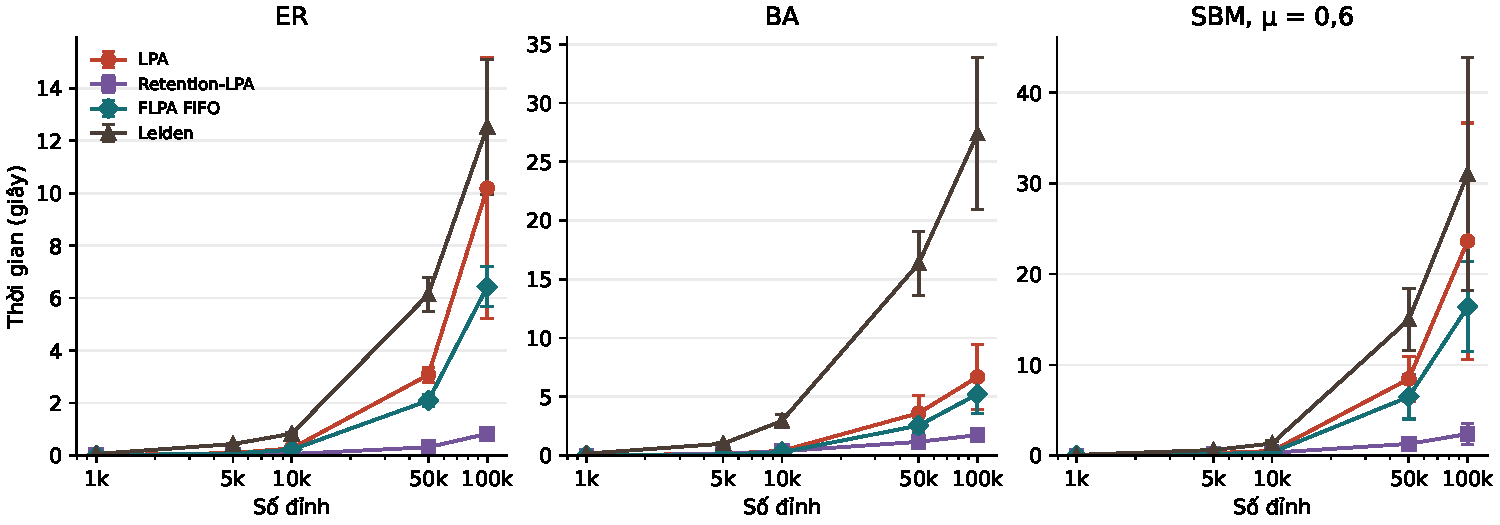
\includegraphics[width=.94\textwidth]{runtime.pdf}
\caption{E1. Thời gian theo kích thước đồ thị. Mỗi điểm là trung bình 10 lượt và vạch sai số là $\pm$ một SD mẫu. Trục số đỉnh theo log để nhìn rõ các kích thước nhỏ.}
\label{fig:e1rt}
\end{figure*}

\begin{figure*}[t]
\centering
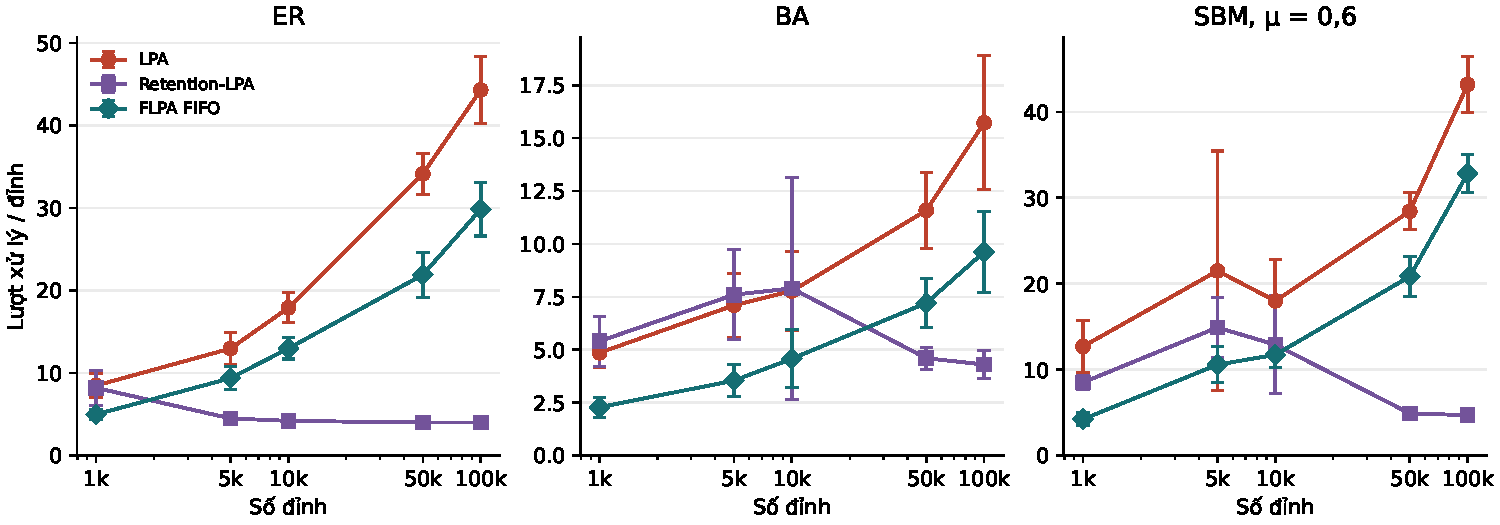
\includegraphics[width=.94\textwidth]{work.pdf}
\caption{E1. Số lượt xử lý trên mỗi đỉnh, kể cả kiểm tra dừng của LPA. Leiden không có bộ đếm này.}
\label{fig:e1work}
\end{figure*}

\begin{table}[t]
\centering
\caption{E1 ở 100.000 đỉnh. Thời gian là mean $\pm$ SD, số lượt và số cụm là mean.}
\label{tab:e1}
\resizebox{\columnwidth}{!}{\EoneTable}
\end{table}

\begin{table}[t]
\centering
\caption{E1 ở 50.000 đỉnh. Điểm Figure 1 xấp xỉ, sai số đọc khoảng 0,05 giây.}
\label{tab:paper}
\resizebox{\columnwidth}{!}{\PaperTable}
\end{table}

\begin{table}[t]
\centering
\caption{Python và mã C tác giả trên cùng đồ thị 100.000 đỉnh và cùng seed số.}
\label{tab:author}
\resizebox{\columnwidth}{!}{\AuthorTable}
\end{table}

E1 hoàn thành 600/600 lượt trên 15 cấu hình. Hình~\ref{fig:e1rt} cho thấy runtime tăng cùng kích thước trong ba họ đồ thị. Hình~\ref{fig:e1work} đối chiếu số lượt xử lý đỉnh. Bảng~\ref{tab:e1} tóm tắt các cấu hình 100.000 đỉnh. LPA và FLPA có cùng bước tính phiếu. Bên cạnh số lượt, phân bố bậc tại các đỉnh được ghé và lần quét để đưa lại láng giềng cũng ảnh hưởng thời gian.

Trên ER 100.000 đỉnh, LPA dùng trung bình 44,30 lượt trên một đỉnh, còn FLPA dùng 29,84. Thời gian trung bình lần lượt là 10,190 và 6,435 giây. Trung bình tỷ lệ ghép cặp LPA/FLPA là $1.58\pm0.69$. Ở mỗi seed, cả hai trả về một cụm lớn cùng một nhãn riêng cho từng đỉnh cô lập. Vì vậy số cụm trung bình 6,3 chủ yếu phản ánh chính sách giữ isolate. Retention-LPA dừng ở trung bình 0,831 giây và trả hơn 31.000 nhóm. Tốc độ của retention đi cùng một nghiệm rất mịn, cũng là xu hướng tác giả quan sát trên ER.

Trên BA 100.000 đỉnh, LPA và FLPA cùng trả một cụm ở cả 10 lần, với thời gian lần lượt $6.679\pm2.780$ và $5.223\pm1.672$ giây. Trung bình tỷ lệ ghép cặp là $1.30\pm0.34$. FLPA giảm lượt đỉnh từ 15,73 xuống 9,62 lượt trên đỉnh. Quét lại láng giềng khi cập nhật hub vẫn có chi phí đáng kể. Retention-LPA tạo khoảng 27.403 cụm trung bình. Leiden thu được trung bình 21,9 cụm và $Q=0.295$. Do BA thiếu nhãn chuẩn, số cụm và modularity cho thấy các dạng phân hoạch khác nhau và làm rõ ảnh hưởng của mục tiêu tối ưu.

SBM 100.000 đỉnh có bậc trung bình thực từ 9,984 đến 10,025 và phần cạnh ngoại khối từ 0,5994 đến 0,6013. Tỷ lệ thời gian LPA/FLPA là $1.40\pm0.54$ theo cặp. LPA và FLPA lần lượt có khoảng 43,18 và 32,83 lượt xử lý trên mỗi đỉnh. Cả hai có NMI xấp xỉ 0 và ACC xấp xỉ 0,01 tại $\mu=0.60$. Retention-LPA cho NMI 0,508 trong khi ARI là 0,0015 và ACC là 0,0059 với hơn 31.000 cụm. Các mảnh nhỏ mang thông tin về nhóm gốc theo NMI, nhưng rất ít cặp cùng nhóm được giữ và các mảnh dư bị phạt khi ghép một-một. Leiden đạt modularity 0,303 trên cấu hình này và NMI 0,021. Hai mục tiêu chất lượng đánh giá những đặc tính khác nhau của phân hoạch.

Bảng~\ref{tab:paper} đưa ra thời gian Figure~1 tại 50.000 đỉnh và độ lệch tương đối của bản Python. Gọi $\bar t_P$ là mean đo được bằng Python và $\bar t_R$ là mean tham chiếu từ hình hoặc phép đo C. Cột sai lệch dùng phần trăm
\begin{equation}
  \Delta = 100\left(\frac{\bar t_P}{\bar t_R}-1\right).
  \label{eq:deviation}
\end{equation}
Điểm tham chiếu từ hình được làm tròn đến 0,05 giây. Độ lệch tương đối dễ nhạy với sai số đọc khi $\bar t_R$ nhỏ. Panel tăng kích thước cắt một số điểm lớn, nên so sánh SBM 100.000 đỉnh tại $\mu=0.60$ sử dụng panel thay đổi $\mu$. Ở panel đó, thời gian LPA và FLPA xấp xỉ 5,80 và 2,70 giây, tỷ số khoảng 2,15. Thử nghiệm Python cho tỷ số của hai mean là 1,44 và mean các tỷ số ghép là 1,40. Cả ba họ đều cho FLPA nhanh hơn LPA theo trung bình ghép cặp ở tất cả kích thước, trong khoảng 1,20–2,46 lần. Độ lớn cải thiện khác nhau theo họ và kích thước. Mốc trên 700 lần trong bài báo thuộc mạng us-patents, được báo cáo ở Bảng~2~\cite{flpa}.

Bảng~\ref{tab:author} bổ sung phép đo trên cùng topology bằng mã C. Cả 54 lượt C hoàn thành ở hai kích thước 10.000 và 100.000. Tại 100.000 đỉnh, tỷ số mean LPA/FLPA của C là 1,98 trên ER, 2,50 trên BA và 2,39 trên SBM. Trên đúng ba cặp seed, thời gian FLPA Python/C có tỷ số mean lần lượt 4,49, 12,93 và 18,06. Ở SBM, FLPA của cả hai backend đều có NMI xấp xỉ 0,0001. Retention-LPA ở cả hai backend trả khoảng 31.000 cụm và có NMI gần 0,509. Hai kết quả này cho thấy hiện tượng gộp cụm và phân mảnh cũng xuất hiện ở mã tham chiếu cùng đồ thị.

Phép so sánh C giữ nguyên cạnh và seed số trên cùng máy Apple M1. Hai backend có thể khác RNG, thứ tự duyệt, cấu trúc lưu trữ và chi phí bộ đếm. Chênh lệch với Figure~1 còn chịu ảnh hưởng của Xeon E5-2697, số lần lặp 10 và 2.000, generator và phiên bản thư viện. Khi đánh giá độ lớn của lợi ích FLPA, cần đọc cả độ lệch chuẩn, số lượt xử lý và kiểu phân hoạch mà mỗi thuật toán tạo ra.


\subsection{E3 — ablation thứ tự và quy tắc đưa lại}
\label{sec:e3}

\begin{figure*}[t]
\centering
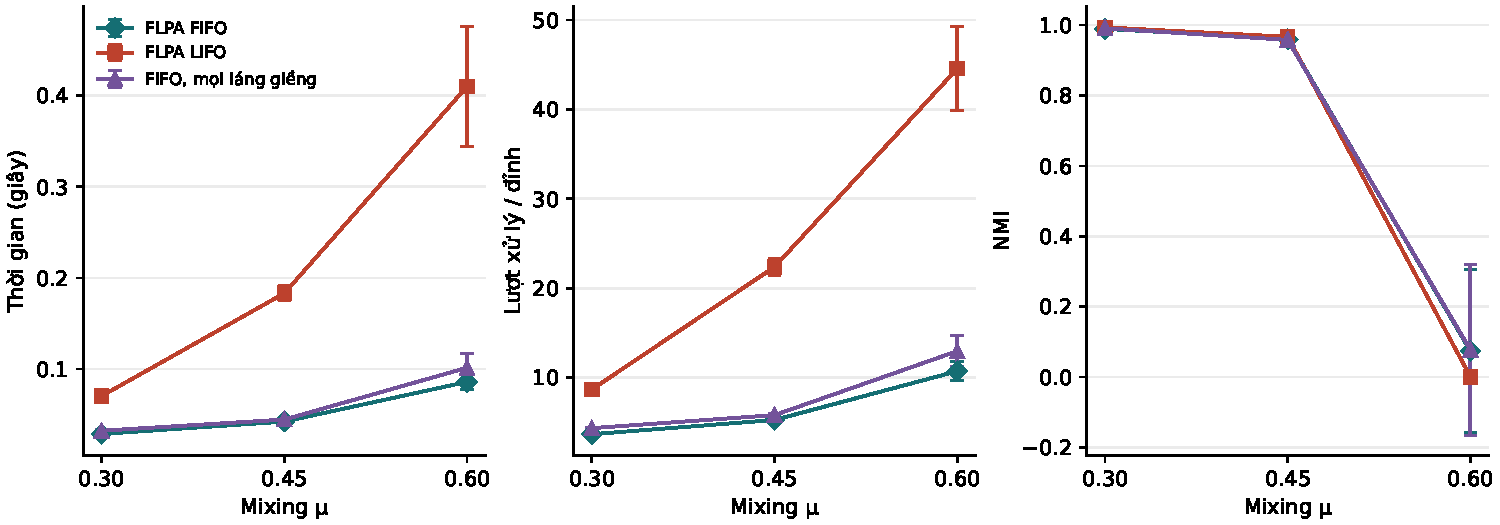
\includegraphics[width=.94\textwidth]{ablation.pdf}
\caption{E3. Chi phí và NMI của ba biến thể FLPA trên SBM 5.000 đỉnh. Điểm là mean và vạch là $\pm$ một SD mẫu trong 10 lần.}
\label{fig:e3}
\end{figure*}

\begin{table*}[t]
\centering
\caption{E3. Chất lượng, công việc và thời gian. Thời gian và các chỉ số có nhãn là mean $\pm$ SD, còn lượt, đổi nhãn và số cụm là mean. Mọi biến thể đều hoàn thành 10/10 cho mỗi $\mu$ và qua kiểm tra maximality.}
\label{tab:e3}
\EthreeTable
\end{table*}

Hình~\ref{fig:e3} và Bảng~\ref{tab:e3} so sánh ba biến thể trên 90 lượt hoàn thành. Thay \texttt{popleft} bằng \texttt{pop} làm lịch xử lý thiên về láng giềng vừa được đưa lại. Cùng một hoán vị ban đầu, LIFO bắt đầu từ đầu còn lại của hàng đợi. Chọn cùng seed và cùng quy tắc phá hoà làm hai biến thể tái lập được trong riêng mỗi lịch, nhưng sau khi thứ tự xử lý khác nhau, thứ tự lấy số ngẫu nhiên cũng khác. Đối chiếu enqueue-all giữ FIFO và cho mọi láng giềng chưa chờ xử lý trở lại hàng đợi sau một cập nhật.

Tại $\mu=0.30$, LIFO xử lý trung bình 43.296 lượt so với 18.293 ở FIFO, đổi nhãn xấp xỉ gấp đôi và tốn thời gian trung bình ghép cặp gấp $2.45\pm0.14$ lần. Chất lượng theo ACC tăng từ 0,966 lên 0,985, với số nhóm trung bình 100,2 sát 100 nhóm thật. Tại $\mu=0.45$, chi phí LIFO tăng lên $4.34\pm0.23$ lần, còn ACC tăng khoảng 0,023 trong khi NMI tăng khoảng 0,006. Cả hai lịch tìm được cấu trúc rõ ở hai mức này. Chất lượng nhích lên có thể có giá trị tùy mục tiêu, nhưng cần cân nhắc số lượt xử lý tăng.

Tại $\mu=0.60$, tỷ lệ thời gian LIFO/FIFO ghép cặp là $4.82\pm0.91$ theo~\eqref{eq:speedup}. LIFO quy về một cụm ở 10/10 lần, với NMI và ARI bằng 0, ACC bằng 0,01. FIFO dự đoán 12,4 cụm trung bình, NMI chỉ 0,073, thể hiện khó khôi phục 100 khối trong cấu hình này. Mỗi biến thể vẫn có maximality 100\% trong các lượt hoàn thành. Một cơ chế phù hợp là LIFO ưu tiên kéo dài quỹ đạo của nhóm đỉnh vừa đổi, dẫn tới bành trướng nhãn trong đồ thị nhiều cạnh giữa nhóm. Ablation đo kết quả và công việc. Kiểm tra cơ chế này sẽ cần trace chi tiết của từng diễn tiến nhãn.

Bỏ điều kiện lọc và đưa lại mọi láng giềng làm số lượt tăng lần lượt khoảng 3.387, 2.706 và 11.234 ở ba mức $\mu$, còn thời gian ghép cặp tăng khoảng 12,4\%, 5,4\% và 18,9\%. Chênh lệch NMI trung bình đều dưới 0,004 theo trị tuyệt đối. Bốc lại nhãn trong thế hoà có thể tạo quỹ đạo mới và đưa thuật toán đến một phân hoạch maximal khác. Kết quả trên ba cấu hình gợi ý rằng lọc chọn láng giềng giảm đánh giá lại, với dao động nhỏ về chất lượng trong mẫu này. E3 chỉ thay một yếu tố mỗi lần trên một họ đồ thị và một kích thước, nên tác động của LIFO lên hub BA hoặc mạng email vẫn cần phép đo riêng.

\subsection{Phần thực nghiệm tích hợp của TV2}
Figure~4 trái của bài báo dùng SBM 100.000 đỉnh và khảo sát NMI theo $\mu$. Bài báo tường thuật giảm độ khôi phục quanh $\mu=0.4$ đến $0.5$~\cite{flpa}. E3 hiện tại dùng 5.000 đỉnh và được thiết kế để đánh giá variant hàng đợi. E2 của TV2 cần đo đủ sweep Figure~4, còn E4 cần đánh giá trên mạng email-Eu-core với nhãn phòng ban. Các bảng và kết luận nhóm về E2/E4 phụ thuộc vào kết quả thực nghiệm từ TV2.

\section{Kết luận}

Việc cài đặt độc lập làm rõ ba cơ chế dừng. LPA yêu cầu toàn bộ nhãn cực đại sau một lượt quét. Retention-LPA khai thác một lượt không đổi. FLPA chỉ đánh giá lại các đỉnh mà lân cận có thể làm giảm ưu thế của nhãn đang giữ. Kiểm thử trên graph điển hình và thực nghiệm kiểm được maximality của những lượt hoàn thành. Giao thức chung cho phép đối chiếu thời gian và lượt xử lý thay vì suy đoán lợi ích chỉ từ tên thuật toán.

E1 ghi nhận lợi ích của lịch FIFO so với quét toàn bộ LPA và đồng thời cho thấy Retention-LPA có thể dừng nhanh khi tạo phân hoạch mịn. E3 cho thấy đổi trật tự xử lý làm thay đổi cả công việc lẫn số cụm, đặc biệt khi SBM khó phục hồi. Chúng tôi công bố seed, trạng thái dừng và dữ liệu thô để có thể kiểm những kết luận này. Tích hợp E2 và E4 sẽ bổ sung kiểm chứng chất lượng tại quy mô Figure~4 và khả năng khái quát sang liên lạc thực tế.

\bibliographystyle{IEEEtran}
\bibliography{references}
\end{document}
